\documentclass[conference]{IEEEtran}
\IEEEoverridecommandlockouts
\usepackage{cite}
\usepackage[utf8]{inputenc}
\usepackage[english]{babel}
\usepackage{bookmark}
\usepackage[square,sort,comma,numbers]{natbib}
\usepackage{listings}
\usepackage{url}
\usepackage{wrapfig}
\usepackage{caption}
\usepackage{color}
\usepackage{enumitem}
\usepackage{graphicx}
\usepackage{float}
\usepackage{url}
\def\UrlBreaks{\do\/\do-}
\usepackage{breakurl}
\graphicspath{{images/}}
\usepackage{hyperref}


\def\BibTeX{{\rm B\kern-.05em{\sc i\kern-.025em b}\kern-.08em
T\kern-.1667em\lower.7ex\hbox{E}\kern-.125emX}}

\date{April 14, 2019}

\makeatletter
\let\thedate\@date


\definecolor{codegreen}{rgb}{0,0.6,0}
\definecolor{codegray}{rgb}{0.5,0.5,0.5}
\definecolor{codepurple}{rgb}{0.58,0,0.82}
\definecolor{backcolour}{rgb}{0.95,0.95,0.92}

\lstdefinestyle{mystyle}{
    backgroundcolor=\color{backcolour},   
    commentstyle=\color{codegreen},
    keywordstyle=\color{magenta},
    numberstyle=\tiny\color{codegray},
    stringstyle=\color{codepurple},
    basicstyle=\scriptsize,
    breakatwhitespace=false,         
    breaklines=true,                 
    captionpos=b,                    
    keepspaces=true,                 
    numbers=left,                    
    numbersep=5pt,                  
    showspaces=false,                
    showstringspaces=false,
    showtabs=false,                  
    tabsize=2
}
    
\lstset{style=mystyle}

\begin{document} 
    \title{
        Crime Prediction using Deep Learning\\[0.3cm]
        \large Interim Report\\
        ELE494-09
    }

    \author{
        \IEEEauthorblockN{Yousif Khaireddin}
        \IEEEauthorblockA{b00063618}
        \and
        \IEEEauthorblockN{Nasir Khalid}
        \IEEEauthorblockA{b00065082}
    }

    \maketitle

    \section{Objective}

    The objective of our project is to develop a trained neural network
    that is capable of predicting within the city of Vancouver. 
    We will be implementing multiple different architectures and
    evaluating their performance.

    \section{Model, Inputs and Outputs}

    As of now we have developed two models to help in crime prediction. We plan on
    developing a few more as well as tweaking the existing ones (more on this in
    future work section). The developed models and their results can be seen through the link included in the references \cite{project}. 
    The two models developed are outlined below:

    \subsection{Model 1}

    This model takes date and time as input. The output is the neighborhood most
    likely to have crime at that moment. The input shape will be [1 x 5] where each
    row is a crime and the 5 columns are:

    \begin{enumerate}
        \item Year
        \item Day
        \item Month
        \item Hour
        \item Minute
    \end{enumerate}

    The output is a [1 x 22] vector where each of the columns represents one of the
    22 neighborhoods in Vancouver. They are listed in the appendix in section I. The
    probabilities of crime happening at the given input time and date are distributed
    across the 22 columns (neighborhoods)

    \subsection{Model 2}

    This model takes date, time and neighborhood as an input. It outputs the probability
    of a crime taking place. The input shape will be [1 x 6]. Where each row is a crime
    and the 6 columns are:

    \begin{enumerate}
        \item Year
        \item Day
        \item Month
        \item Hour
        \item Minute
        \item Neighborhood
    \end{enumerate}

    The output is a [1 x 2] vector where the first index contains the probability of
    crime occurring where as the second index is the probability of no crime.
    
    \section{Datasets}

    For the project we obtained all of our data from the city of
    Vancouvers open data source \cite{DT}. The first dataset we
    obtained from the website was the crime dataset \cite{DT_C}.
    The columns of the dataset were the following:\\

    \begin{enumerate}
        \item Type of crime
        \item Year
        \item Day
        \item Month
        \item Hour
        \item Minute
        \item Block of crime
        \item Neighborhood of crime
        \item X Co-ordinate of crime in UTM Zone 10
        \item Y Co-ordinate of crime in UTM Zone 10
        \item Latitude
        \item Longitude\\
    \end{enumerate}

    The entire dataset consisted of 530652 crimes from 2003 to 2017. However for some of the them
    their time and location data was missing as it was protected for privacy reasons.
    This data was essentially useless for us so we eliminated all of these crimes and
    that left us with a total of 476290 crimes to work with.\\
    
    We then downloaded a second dataset from the Vancouver open data catalogue that
    gave us a list of neighborhoods in Vancouver \cite{DT_N}. We added 2 new columns
    to this dataset called 'Latitude' and 'Longitude' and in here we added the center
    latitude and longitude for each respective neighborhood. This second dataset
    consisted of the following columns:\\

    \begin{enumerate}
        \item Map ID
        \item Name
        \item Latitude (Added)
        \item Longitude (Added)\\
    \end{enumerate}

    \section{Dataset Preprocessing}

    We used to Pandas library to work with the .csv files that we had imported. We wrote a seperate
    python file that is attatched in appendix B to create a seperate column in our crime dataset called
    neighborhood. The difference between our added column and the existing column is that our list of neighborhoods
    was extracted from the previously mentioned neighborhoods dataset. Our python script mapped the co-ordinates of every crime
    to the neighborhoods in the second dataset. This is why we had added a latitude and longitude to the neighborhood dataset.
    The neighborhoods we have added are consistent throughout the crime dataset and future datasets we plan to add will also use this
    script\\

    After this we added another new column to the dataset called 'Crime' and we gave all the rows a value
    of 1. This corresponds to the fact that they are all crimes. We then upscaled the data
    to add more time and date entries in between the date and times where they were crimes.
    We gave these rows a 'Crime' value of 0 to indicate that there was no crime at that
    time. Each of the added rows were also given a randomly generated neighborhood as well.
    For example take the tables as a subset of the data before and after:

    \begin{table}[H]
        \renewcommand{\arraystretch}{1.3}
        \caption{Data before Upscaling}
        \label{table_example}
        \centering
        \begin{tabular}{|c|c|c|}
        \hline
        \bfseries Date and Time & \bfseries Crime & \bfseries Neighborhood\\
        \hline
        2017-07-13 20:52:00 & 1 & Sunset\\
        \hline
        2017-07-13 21:30:00 & 1 & Hastings-Sunrise\\
        \hline
        2017-07-13 22:23:00 & 1 & Fairview\\
        \hline
        \end{tabular}
    \end{table}

    \begin{table}[H]
        \renewcommand{\arraystretch}{1.3}
        \caption{Data after Upscaling}
        \label{table_example}
        \centering
        \begin{tabular}{|c|c|c|}
        \hline
        \bfseries Date and Time & \bfseries Crime & \bfseries Neighborhood\\
        \hline
        2017-07-13 20:52:00 & 1 & Sunset\\
        \hline
        2017-07-13 21:00:00 & 0 & Downtown\\
        \hline
        2017-07-13 21:30:00 & 1 & Hastings-Sunrise\\
        \hline
        2017-07-13 22:00:00 & 0 & Sunset\\
        \hline
        2017-07-13 22:23:00 & 1 & Fairview\\
        \hline
        \end{tabular}
    \end{table}

    In this case we have upscaled by a factor of 30 minutes so at every 30 minute mark if
    a date and time do not have a crime then a new entry is added where the crime is 0 and
    a random neighborhood is assigned as well. Through this procedure we increased the total
    number of samples up to 595370 and with the added 'Crime' column the shape of the dataset
    became [595370 x 1 x 13]. We then removed the 'Block of crime', ' X Co-ordinate of crime in UTM Zone 10',
    'Y Co-ordinate of crime in UTM Zone 10' and the 'Neighborhood of crime' from dataset as we did not need these.
    \emph{The removed 'Neighborhood of crime' was the one initially in dataset and NOT the one we added}. Therefore,
    our final dataset has the shape [595370 x 1 x 9]

    \section{Creating Model 1}

    For model 1 we want the output to be the likelihood of crime across all the neighborhoods. So we only want to train it on the entries of the dataset where the 'Crime' value is 1
    or we basically want it to learn only from the crime data. Furthermore the output of the network will not give a yes or no for crime but instead a probability of crime. For these
    reasons we will be training this model only on the time entries where there has been a crime. We start by extracting all the time entries in the dataset where there has been a crime.
    This will shrink our upscaled dataset from 595370 to 476290. From this we extract the needed columns for the input vector which are year, month, day, hour and minute.
    We then tried to normalize the data using the code in Appendix C. After this we extracted the output vector for the model which was the 'Neighborhood' column. We one-hot encoded them. After this
    we split it in to a training set, validation set and a test set. This can be seen in the image output below:

    \begin{figure}[H]
        \centering
        \captionsetup{justification=centering}
        \centering
            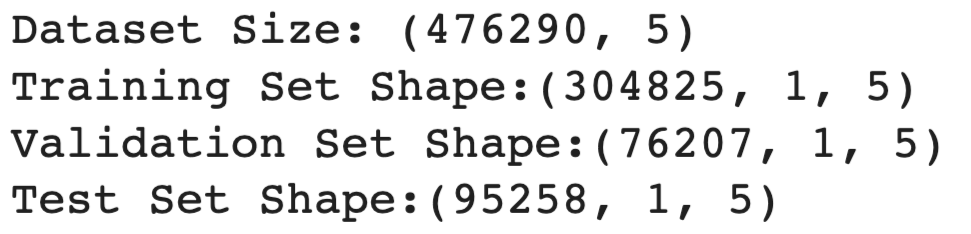
\includegraphics[width=0.4\textwidth]{one1.png}
            \caption{Data split for model 1}
    \end{figure}

    The output vector has 22 columns where one represents each neighborhood. Our network is a sequential model, using a categorical crossentropy loss function and rmsprop optimizer. Activation functions are relu except the finl softmax layer. Its summary is shown below:

    \begin{figure}[H]
        \centering
        \captionsetup{justification=centering}
        \centering
            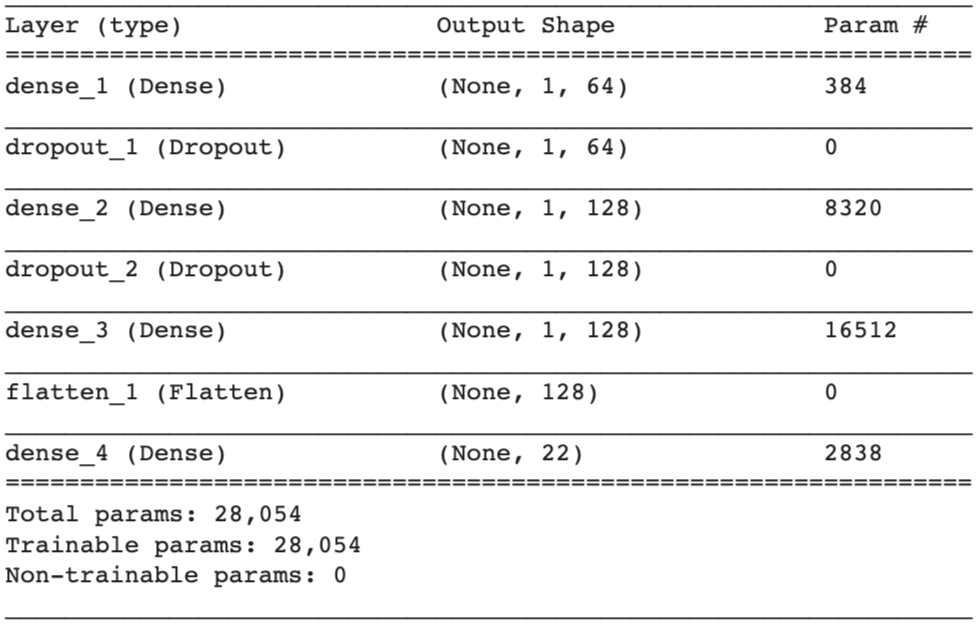
\includegraphics[width=00.5\textwidth]{m1.png}
            \caption{Summary for model 1}
    \end{figure}

    We trained it for 20 epochs with a batch size of 150. The final training accuracy was 22\% and the validation accuracy
    was 21.8\%. On the test set the accuracy was 21.84\%. Shown below is a plot of of the change in validation and training loss across epochs.

    \begin{figure}[H]
        \centering
        \captionsetup{justification=centering}
        \centering
            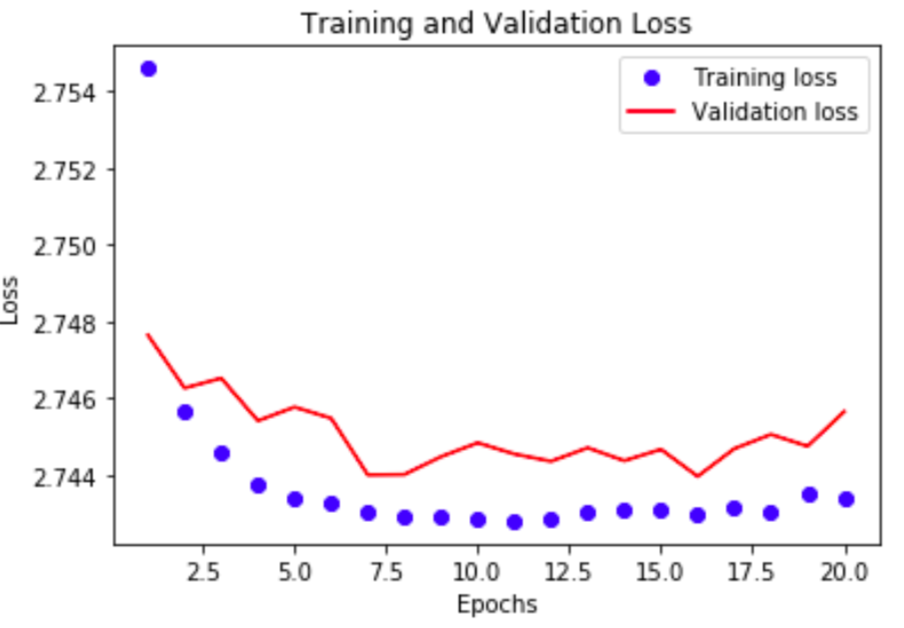
\includegraphics[width=0.4\textwidth]{m1_t.png}
            \caption{Validation and Training loss across epochs for Model 1}
    \end{figure}

    \section{Creating Model 2}

    For this model we want the output to be either a 1 or 0 to indicate that a crime will happen or it wont. For this reason the output used to train the network
    will be the 'Crime' column. The input to the network will be year, month, day, time, hour and neighborhood. For these reasons we will use the entire dataset so
    that the network can also learn from cases where there is no crime. We also perform some normalization on this input data using the code in Appendix D. Our dataset is of size 595370 and from this we begin by extracting
    the needed input columns and splitting them in to the training, validation and test sets. This is shown below:

    \begin{figure}[H]
        \centering
        \captionsetup{justification=centering}
        \centering
            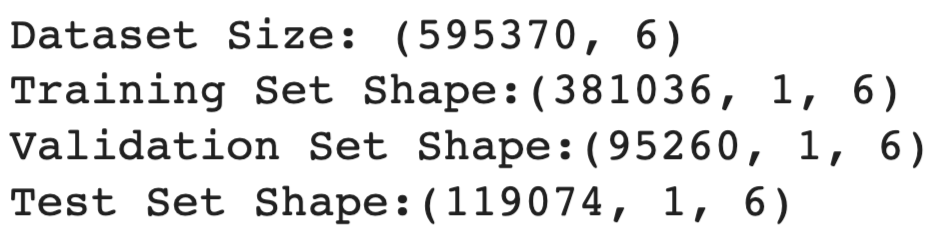
\includegraphics[width=0.4\textwidth]{m2.png}
            \caption{Data split for model 2}
    \end{figure}

    The output vector has only two columns either 1 or 0 (crime or no crime) and therefore we use a binary-cross entropy loss function along with rmsprop here to train the network. Activation functions are relu except the finl softmax layer. The
    network summary is shown below:

    \begin{figure}[H]
        \centering
        \captionsetup{justification=centering}
        \centering
            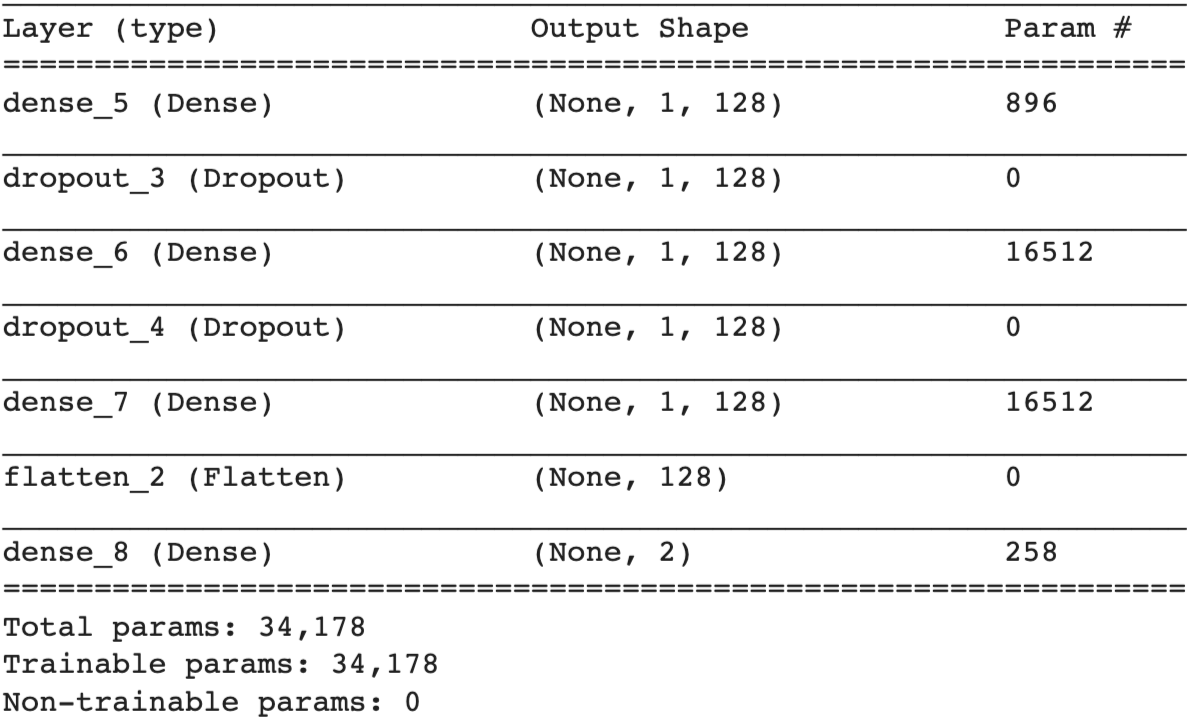
\includegraphics[width=0.5\textwidth]{m2_s.png}
            \caption{Summary for model 1}
    \end{figure}

    We trained it for 20 epochs with a batch size of 150. The final training accuracy was 84.21\% and the validation accuracy
    was 84.62\%. On the test set the accuracy was 84.67\%. Shown below is a plot of of the change in validation and training loss across epochs.

    \begin{figure}[H]
        \centering
        \captionsetup{justification=centering}
        \centering
            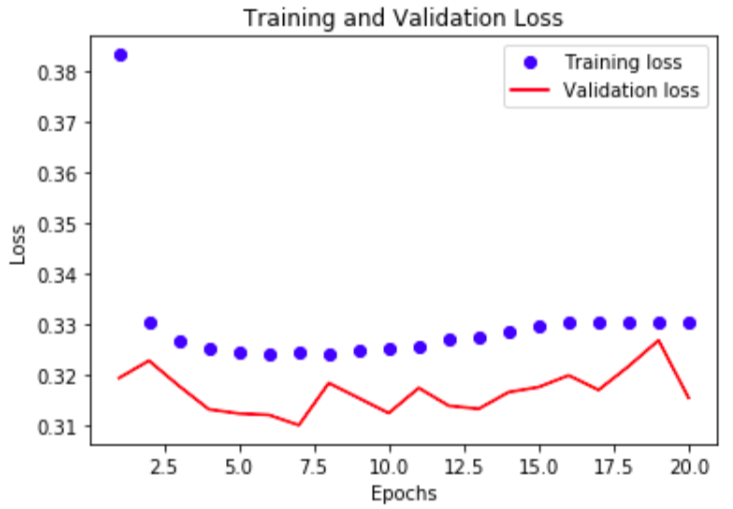
\includegraphics[width=0.4\textwidth]{m2_t.png}
            \caption{Validation and Training loss across epochs for Model 2}
    \end{figure}

    \section{Future Work}

    We plan to upgrade our existing models to improve accuracy as well as implement a recurrent neural network that can better account for the time dependency
    in the data. Furthermore, based on the reading we were assigned we also want to implement the walk-forward optimization outlined in the reference paper \cite{ref}.
    This is so we train our data on a set that it can also evaluate on which is not too far apart in terms of year. Therefore it would better to learn using walk-forward
    
    \begin{figure}[H]
        \centering
        \captionsetup{justification=centering}
        \centering
            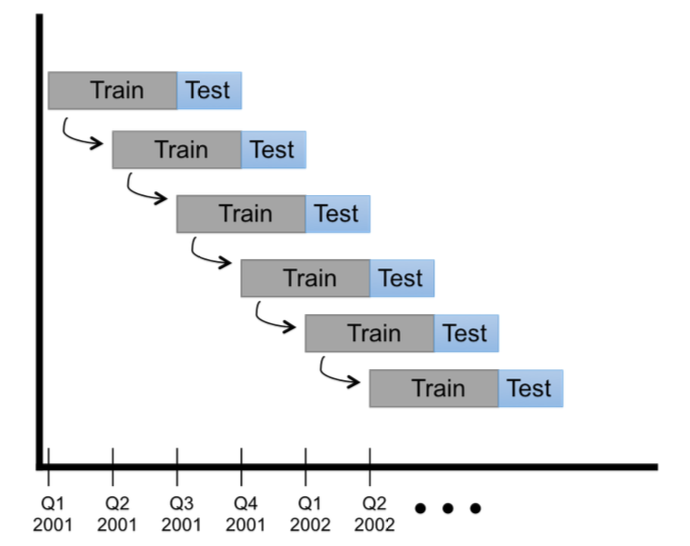
\includegraphics[width=0.35\textwidth]{train.png}
            \caption{Diagram of walk-forward optimization during training \cite{ref}}
    \end{figure}

    Furthermore, we are also going to add more data to our existing dataset. From the Vancouver data catalogue we will be adding weather data to the dataset however we also noticed
    that they have data on the following \cite{DT}:\\

    \begin{enumerate}
        \item Location of Alleyways
        \item Location of Cultural Spaces
        \item Location of Bikeracks
        \item Location of Graffitis
        \item Location of Washrooms
        \item Location of Schools
        \item Location of Drinking Fountains
        \item Location of Community centres
        \item Location of Railways\\
    \end{enumerate}
    
    We want to use this data along with our existing crime dataset. In the case of weather we would add the weather conditions at the time of the crime. However, we also want to add additional
    data about the distance of the crime from the location of nearest schools, cultural spaces, graffiti etc which is available on the data catalogue. Through this we hope to account for spatial information
    around the city without having to explicitly use a convolutional neural network.

    \newpage

    \bibliographystyle{IEEEtran}
    \bibliography{report}

    \appendix

    \subsection{Neighborhoods in Vancouver}
    \begin{enumerate}
        \item Sunset
        \item Mount Pleasant
        \item Riley Park
        \item Downtown
        \item Kitsilano
        \item Dunbar-Southlands
        \item Kerrisdale
        \item Arbutus-Ridge
        \item West Point Grey
        \item Marpole
        \item Oakridge
        \item Shaughnessy
        \item Fairview
        \item South Cambie
        \item West End
        \item Killarney
        \item Renfrew-Collingwood
        \item Hastings-Sunrise
        \item Victoria-Fraserview
        \item Kensington-Cedar Cottage
        \item Strathcona
        \item Grandview-Woodland
    \end{enumerate}

    \subsection{Python script to add new neighborhood column to crime dataset}

    \begin{lstlisting}[language=Python, caption=Neighborhood Column Adder]
import pandas as pd
import numpy as np

file_path = '../Datasets/cov_localareas.csv'
file_path2 = '../Datasets/crime.csv'

df_localareas = pd.read_csv(file_path)
df_crimes = pd.read_csv(file_path2)

df_crimes = df_crimes[['Latitude', 'Longitude']] 

data = np.empty_like(df_crimes['Latitude'],dtype='<U24')

df_crimes = df_crimes.values
location_cords = df_localareas[
                    ['Latitude', 'Longitude']].values
addresses = df_localareas['NAME'].values

for n, i in enumerate(df_crimes):
    data[n] = addresses[np.argmin(np.sum(np.square(i-location_cords), axis=1))]
print(data)
print(data.shape)

final_crime = pd.read_csv(file_path2)
final_crime['Neighbourhood'] = data
final_crime.to_csv('../Datasets/final_crime.csv', index=False)\end{lstlisting}


\subsection{Normalization of inputs for model 1}

\begin{lstlisting}[language=Python, caption=Normalizing Input of model 1]
X_1[:, 0] *= 1/10000  # Year
X_1[:, 1] *= 1/12     # Month
X_1[:, 2] *= 1/31     # Day
X_1[:, 3] *= 1/24     # Hour
X_1[:, 4] *= 1/60     # Minute\end{lstlisting}

\subsection{Normalization of inputs for model 2}

\begin{lstlisting}[language=Python, caption=Normalizing Input of model 2]
X_2[:, 0] *= 1/10000  # Year
X_2[:, 1] *= 1/12     # Month
X_2[:, 2] *= 1/31     # Day
X_2[:, 3] *= 1/24     # Hour
X_2[:, 4] *= 1/60     # Minute
X_2[:, 5] *= 1/23.0   # Neighbourhood\end{lstlisting}

\end{document}